\documentclass[../main.tex]{subfiles}

    \begin{document}
    \newpage

%%%%%%%%%%%%%%%%%%%%%%%%%%%%%%%%%%%%%%%%%%
    % Thématique urbanisme
    \vspace{15pt}
    \noindent
    \Large
\textbf{\textcolor{UGEblue}{~Thématique~3~:}}
    \\
\colorbox{UGEblue}{\textbf{\textcolor{white}{~Agencer l'organisation territoriale de la région~}}}
    \vspace{15pt}

%%%%%%%%%%%%%%
    % Volet
    \vspace{15pt}
    %\needspace{20pt} % Réserve de l'espace
\section{Densifier et diversifier}

    % Block
\begin{block}[Intervenir]
    \linespread{0.9}\selectfont % Réduit l'interligne
    \emoji{houses} % Emoji
    \textit{\small{Intervenir sur les activités et sur le bâti afin de densifier et de diversifier les usages.}}
\end{block}

    \begin{multicols}{2}
    \raggedcolumns
    \small{
L’intervention sur le bâti et les activités dans les quartiers de gare permet de structurer un développement urbain \gras{plus dense et plus mixte}, favorable au système de mobilité alternatif. Il ne s’agit pas seulement d’augmenter \gras{la densité résidentielle et d’emplois}, mais aussi \gras{de diversifier les destinations}, basées sur une offre d'équipements et de services de proximité, en adéquation avec les principes de la «~ville du quart d'heure~».
    \\\\
Ces opérations d'aménagement visent à rendre les quartiers de gare \gras{plus attractifs}, où l’accès aux commerces, aux services publics et aux espaces de sociabilité limite la dépendance aux déplacements motorisés. En promouvant l'usage intermodal du vélo et de la micro-mobilité, \gras{65~\% de la population} régionale bénéficie ainsi d'un accès à un point d'arrêt du réseau ferroviaire, tandis que \gras{70~\% des emplois} et \gras{75~\% des points d'intérêt} du périmètre régional deviennent accessibles.
    }
    %\\\\
\begin{center}
    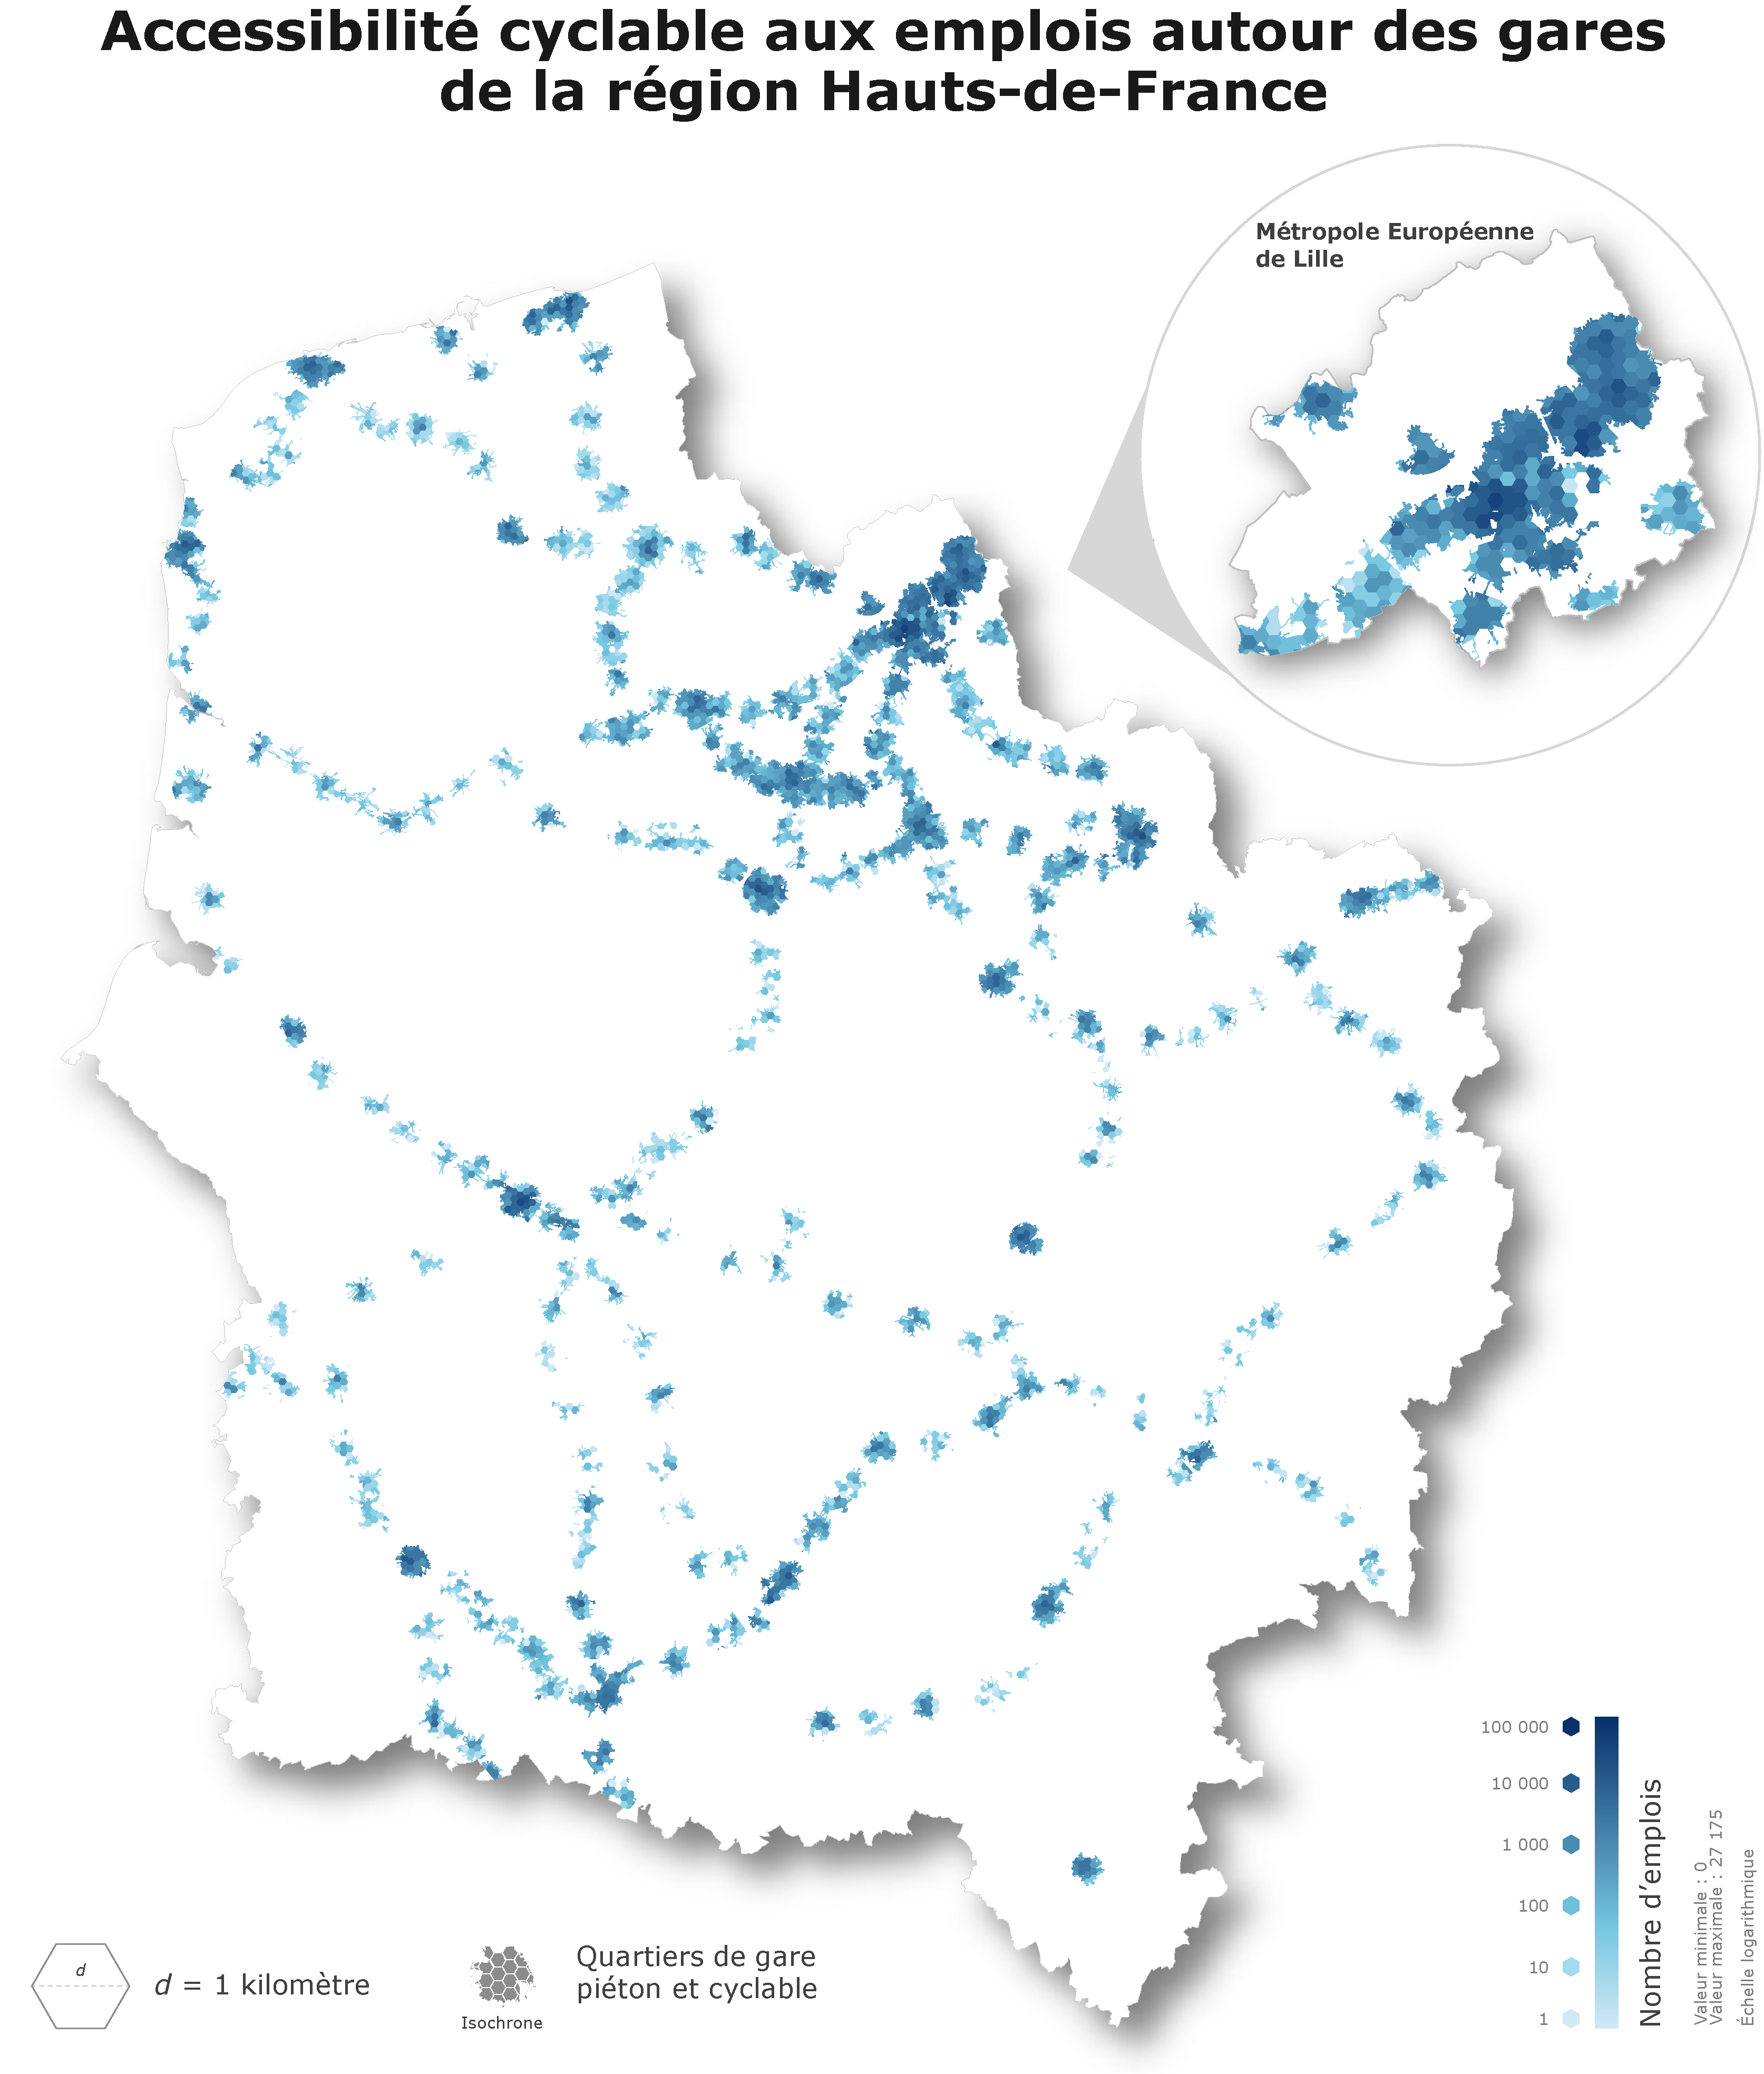
\includegraphics[width=\columnwidth]{figures/policy-brief-carte-emplois-compresse.pdf}
    \label{acces-emplois}
    \vspace{-0.5cm}
    \begin{flushright}
            \scriptsize{\textcolor{darkgray}{Auteur~: Dylan Moinse (2025)}}
    \end{flushright}
\end{center}

    \end{multicols}

    \end{document}